% ------------------------------------------------------------------------------
% TYPO3 CMS 8.0 - What's New - Chapter "Introduction" (English Version)
%
% @author	Michael Schams <schams.net>
% @license	Creative Commons BY-NC-SA 3.0
% @link		http://typo3.org/download/release-notes/whats-new/
% @language	English
% ------------------------------------------------------------------------------
% LTXE-CHAPTER-UID:		cb43d098-7bf9a537-bf3817c0-53a0f29f
% LTXE-CHAPTER-NAME:	Introduction
% ------------------------------------------------------------------------------

\section{Introduction}
\begin{frame}[fragile]
	\frametitle{Introduction}

	\begin{center}\huge{Introduction}\end{center}
	\begin{center}\huge{\color{typo3darkgrey}\textbf{The Facts}}\end{center}

\end{frame}

% ------------------------------------------------------------------------------
% LTXE-SLIDE-START
% LTXE-SLIDE-UID:		9e397afb-762f7061-0e0e0bd1-9836250e
% LTXE-SLIDE-TITLE:		TYPO3 CMS 8.0 - The Facts
% ------------------------------------------------------------------------------
\begin{frame}[fragile]
	\frametitle{Introduction}
	\framesubtitle{TYPO3 CMS 8.0 - The Facts}

	\begin{itemize}
		\item Release date: 22 March 2016
		\item Release type: Sprint Release
		\item Slogan: Start your engines
	\end{itemize}

	\begin{figure}
		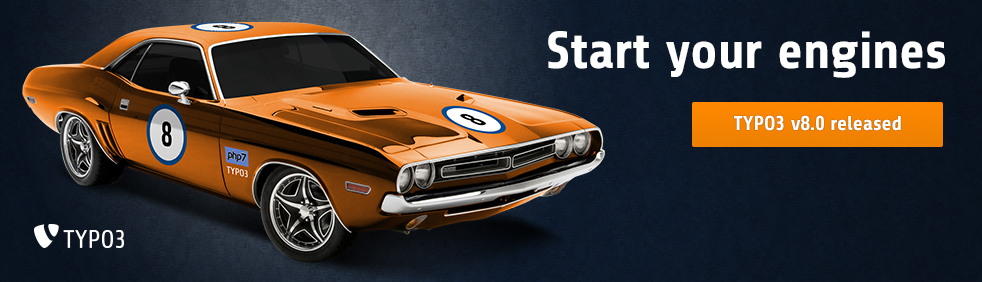
\includegraphics[width=0.95\linewidth]{Introduction/typo3cms80-banner.png}
	\end{figure}

\end{frame}

% ------------------------------------------------------------------------------
% LTXE-SLIDE-START
% LTXE-SLIDE-UID:		737c8e9b-4ae60e26-6975ea72-21146dd0
% LTXE-SLIDE-TITLE:		System Requirements
% ------------------------------------------------------------------------------
\begin{frame}[fragile]
	\frametitle{Introduction}
	\framesubtitle{System Requirements}

	\begin{itemize}
		\item PHP:\tabto{2.2cm}version 7
		\item MySQL:\tabto{2.2cm}version 5.5 to 5.7
		\item Disk space:\tabto{2.2cm}min 200 MB
		\item PHP settings:

			\begin{itemize}
				\item \texttt{memory\_limit} >= 128M
				\item \texttt{max\_execution\_time} >= 240s
				\item \texttt{max\_input\_vars} >= 1500
				\item compilation option \texttt{-}\texttt{-disable-ipv6} must \underline{not} be used
			\end{itemize}

		\item The backend requires Microsoft Internet Explorer 11 or later,
			Microsoft Edge, Google Chrome, Firefox, Safari or any other modern,
			compatible browser

	\end{itemize}

\end{frame}

% ------------------------------------------------------------------------------
% LTXE-SLIDE-START
% LTXE-SLIDE-UID:		90d2d3d1-f9d57661-dd01143b-10630416
% LTXE-SLIDE-TITLE:		Development And Release Timeline
% ------------------------------------------------------------------------------
\begin{frame}[fragile]
	\frametitle{Introduction}
	\framesubtitle{Development and Release Timeline}

	\begin{figure}
		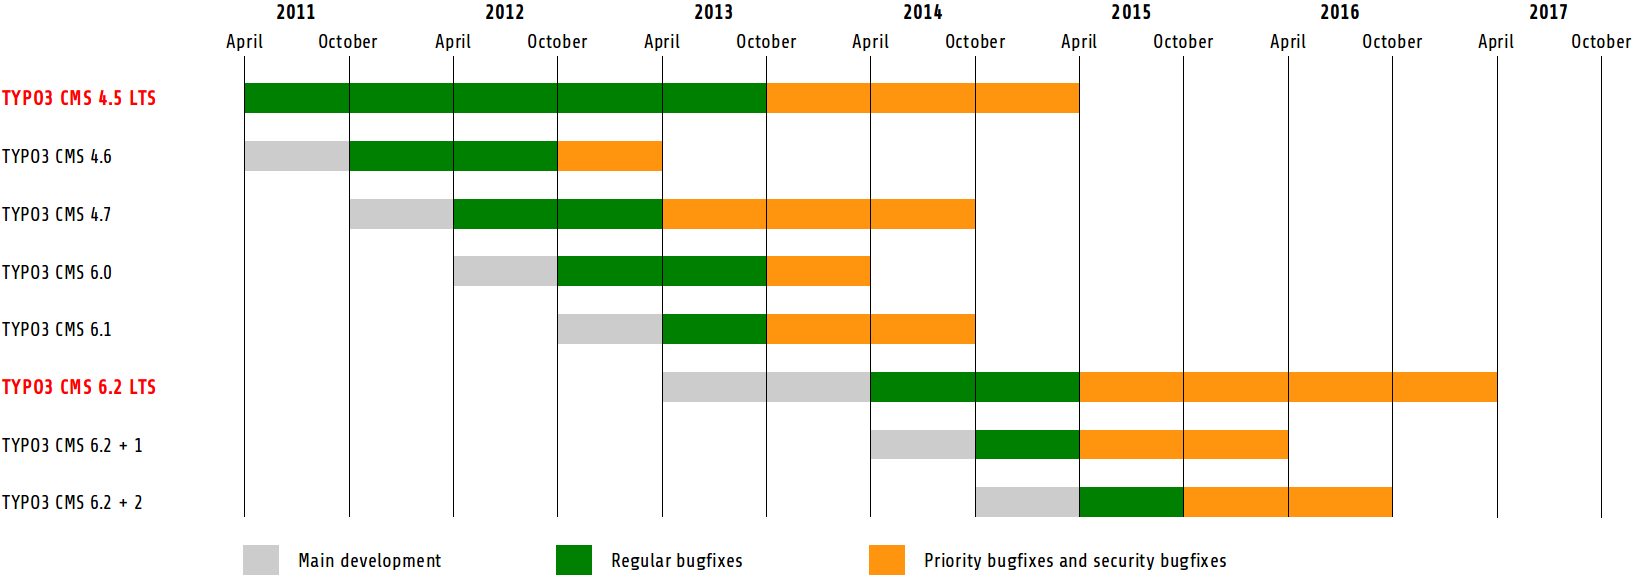
\includegraphics[width=1\linewidth]{Introduction/ReleaseAgenda.png}
	\end{figure}

\end{frame}

% ------------------------------------------------------------------------------
% LTXE-SLIDE-START
% LTXE-SLIDE-UID:		13e0fd6a-fa50d02d-c15c4af0-f3996926
% LTXE-SLIDE-TITLE:		TYPO3 CMS Roadmap
% ------------------------------------------------------------------------------
\begin{frame}[fragile]
	\frametitle{Introduction}
	\framesubtitle{TYPO3 CMS Roadmap}

	Release dates and their primary focus:

	\begin{itemize}

		\item
			\begingroup
				\color{typo3orange}
					v8.0 \tabto{1.1cm}22/Mar/2016\tabto{3.4cm}Adding last minute things
			\endgroup
		\item v8.1 \tabto{1.1cm}03/May/2016\tabto{3.4cm}Cloud Integration
		\item v8.2 \tabto{1.1cm}05/Jul/2016\tabto{3.4cm}Rich Text Editor
		\item v8.3 \tabto{1.1cm}30/Aug/2016\tabto{3.4cm}Frontend Editing on Steroids
		\item v8.4 \tabto{1.1cm}18/Oct/2016\tabto{3.4cm}\textit{to be determined}
		\item v8.5 \tabto{1.1cm}20/Dec/2016\tabto{3.4cm}Integrator Support
		\item v8.6 \tabto{1.1cm}14/Feb/2017\tabto{3.4cm}\textit{to be determined}
		\item v8.7 \tabto{1.1cm}04/Apr/2017\tabto{3.4cm}LTS Preparation

	\end{itemize}

	\smaller
		\url{https://typo3.org/typo3-cms/roadmap/}\newline
		\url{https://typo3.org/news/article/kicking-off-typo3-v8-development/}
	\normalsize

\end{frame}

% ------------------------------------------------------------------------------
% LTXE-SLIDE-START
% LTXE-SLIDE-UID:		06c6100a-69216610-618bde63-bbdc4eef
% LTXE-SLIDE-TITLE:		Installation
% ------------------------------------------------------------------------------
\begin{frame}[fragile]
	\frametitle{Introduction}
	\framesubtitle{Installation}

	\begin{itemize}
		\item Official installation procedure under Linux/Mac OS X\newline
			(DocumentRoot for example \texttt{/var/www/site/htdocs}):
		\begin{lstlisting}
			$ cd /var/www/site
			$ wget --content-disposition get.typo3.org/8.0
			$ tar xzf typo3_src-8.0.0.tar.gz
			$ cd htdocs
			$ ln -s ../typo3_src-8.0.0 typo3_src
			$ ln -s typo3_src/index.php
			$ ln -s typo3_src/typo3
			$ touch FIRST_INSTALL
		\end{lstlisting}

		\item Symbolic links under Microsoft Windows:

			\begin{itemize}
				\item Use \texttt{junction} under Windows XP/2000
				\item Use \texttt{mklink} under Windows Vista and Windows 7
			\end{itemize}

	\end{itemize}
\end{frame}

% ------------------------------------------------------------------------------
% LTXE-SLIDE-START
% LTXE-SLIDE-UID:		b878899c-e4b09ddf-4c0ea575-9e0900ad
% LTXE-SLIDE-TITLE:		Upgrade to TYPO3 CMS 7
% ------------------------------------------------------------------------------
\begin{frame}[fragile]
	\frametitle{Introduction}
	\framesubtitle{Upgrade to TYPO3 CMS 8.x}

	\begin{itemize}
		\item Upgrades only possible from TYPO3 CMS 7.6 LTS
		\item TYPO3 CMS < 7.6 LTS should be updated to TYPO3 CMS 7.6 LTS first
	\end{itemize}

	\begin{itemize}

		\item Upgrade instructions:\newline
			\smaller\url{http://wiki.typo3.org/Upgrade#Upgrading_to_8.0}\normalsize
		\item Official TYPO3 guide "TYPO3 Installation and Upgrading":
			\smaller\url{http://docs.typo3.org/typo3cms/InstallationGuide}\normalsize
		\item General approach:
			\begin{itemize}
				\item Check minimum system requirements \small(PHP, MySQL, etc.)
				\item Review \textbf{deprecation\_*.log} in old TYPO3 instance
				\item Update all extensions to the latest version
				\item Deploy new sources and run Install Tool -> Upgrade Wizard
				\item Review startup module for backend users (optionally)
			\end{itemize}
	\end{itemize}

\end{frame}

% ------------------------------------------------------------------------------

% ------------------------------------------------------------------------------
% LTXE-SLIDE-START
% LTXE-SLIDE-UID:		e4b09ddf-4c0ea575-9e0900ad-b878899c
% LTXE-SLIDE-TITLE:		PHP Version 7
% ------------------------------------------------------------------------------
\begin{frame}[fragile]
	\frametitle{Introduction}
	\framesubtitle{PHP Version 7}

	\begin{itemize}

		\item PHP 7.0 is the minimum requirement for TYPO3 CMS 8.x
		\item TYPO3 will support subsequent PHP 7 releases as they come out
		\item This version raise gives a significant performance boost to the overall system

		\item Not only backend editors will notice a more fluent interface, but the
			new all-time record for a full cached page call in the frontend is below
			7 milliseconds now, which is approximately 40\% faster compared to running
			the very same website with PHP version 5.5

		\item We also started using new features from this PHP version, for instance
			the cryptographically secure pseudo-random generators are in active use already

	\end{itemize}

\end{frame}

% ------------------------------------------------------------------------------
